\chapter{Conclusion}
\label{ch:conclusion}

\begin{figure}
    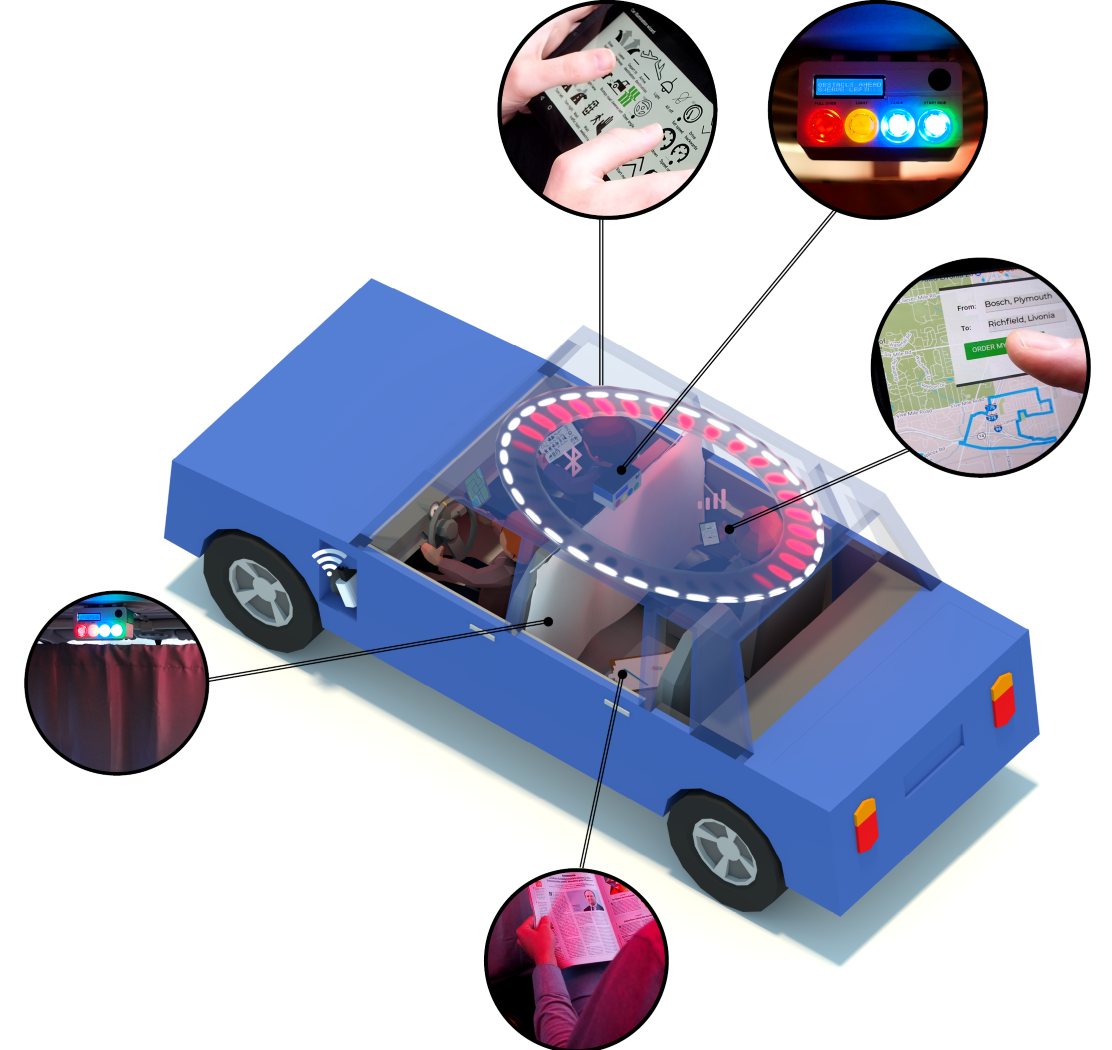
\includegraphics[width=\textwidth]{fig/PosterFigure_1920.png}
    \caption[Overview]{Overview of the realized components for the on-the-road WOz study}
    \label{fig:overview}
\end{figure}

The ambient display is a possibility to assist passengers in autonomous vehicles with noncritical information that is not annoying and guides their attention out of the vehicle onto the road. 
This might help to calm passengers and reduce driving sickness. This display can be integrated naturally and unobtrusively into the ceiling of vehicles. The information catches the attention even if passengers are not focusing directly on it. 

As seen in the \emph{\fullref{sec:videoAnalysis}} participants behaved differently in the conditions, this cannot only be attributed to information from the text display. In fact, a few passengers mentioned that they noticed something but did not see color in their peripheral sight: \say{I noticed something, was going on, and it did, but I cannot recall having seen something}. I conclude that people did not perceive the individual colors much, but their attention was guided by the movements (or change in lightness) of the ambient display (see \emph{\fullref{sec:eye}}). 
Once people were given the light information, they felt irritated when the light display did not light up in similar cases. People who did not have the feedforward information in the second trip reported to miss it more than the other way round. 

There is no reason to believe that people answered falsely; therefore I expect the observed effects to only become stronger in a plausible self-driving car scenario (see \emph{\nameref{ImproveWizard}}) and with the suggested alterations to the display (see \emph{\nameref{ImrpoveDisplay}}).

Besides the feedforward information, such a display can be used to give an autonomous vehicle assistant possibilities to express itself and to indicate places of interest. Of course, such displays primarily use is to light up the whole cabin or individual zones and for mood lighting. 

The wizard of oz study design devised for this thesis is a useful tool to simulate fully autonomous vehicles. In combination with the ride-hailing app and the hidden wizards, it provides uninvolved study participants with a sufficiently believable scenario. 

The concept of lighting integrated driving messages for autonomous vehicles is promising and likely to be discovered by others too. In the future, the ambient display could extend from the inside of the car to the shell with 360° externally mounted LEDs and project these driving information to pedestrians too. 